\documentclass[11pt,a4paper]{article}

%=====================
% PACKAGES
%=====================
\usepackage[utf8]{inputenc}
\usepackage[T1]{fontenc}
\usepackage[margin=1in]{geometry}
\usepackage{lmodern}
\usepackage{microtype}
\usepackage{setspace}
\usepackage{amsmath,amssymb,amsfonts,bm}
\usepackage{physics}
\usepackage{siunitx}
\usepackage{graphicx}
\usepackage{booktabs}
\usepackage[numbers,sort&compress]{natbib}
\usepackage[colorlinks=true,linkcolor=blue,citecolor=blue,urlcolor=blue]{hyperref}

% TikZ for the boundary diagram
\usepackage{tikz}
\usetikzlibrary{arrows.meta,patterns,decorations.pathmorphing,positioning,fit,calc}

%=====================
% GLOBAL TYPESETTING TWEAKS
%=====================
\emergencystretch=2em

% Fix for siunitx and physics package conflict
\AtBeginDocument{\RenewCommandCopy\qty\SI}

%=====================
% MACROS
%=====================
\newcommand{\mpl}{M_{\rm Pl}}
\newcommand{\rs}{r_{\rm s}}
\newcommand{\Geff}{G_{\rm eff}}
\newcommand{\ac}{a_{\rm c}}
\newcommand{\zc}{z_{\rm c}}
\newcommand{\cs}{c_{\rm s}}
\newcommand{\be}{\begin{equation}}
\newcommand{\ee}{\end{equation}}
\newcommand{\dx}{\mathrm{d}}

%=====================
% TITLE
%=====================
\title{\textbf{Condensate Link Framework Bridge: Condensate Formation and Boundary--Driven Wave Compression as the Physical Bridge to an Early Stiffness Boost}}
\author{Rob Skavberg\thanks{Independent Researcher, Calgary, Canada. Contact: \texttt{rob.skavberg@example.org}}}
\date{\today}

%=====================
% DOCUMENT
%=====================
\begin{document}
\maketitle
\doublespacing

\begin{abstract}
We consider the \emph{Condensate Link Framework} (CLF) as a \emph{bridge} between vacuum microphysics and early--Universe cosmology. As the condensate vacuum expands into a proto--vacuum fluid, a \emph{Condensate Boundary} forms and advances. Because the acoustic/phase impedances are mismatched across this interface, waves in the proto--fluid that reach the boundary largely reflect and cannot transmit efficiently; they accumulate and experience \emph{boundary--layer compression}. This compression transiently amplifies short--wavelength fluctuations and creates a brief, localized \emph{mechanical energy reservoir} that boosts $H(a)$ (EDE--like), shrinking the sound horizon and raising the CMB--inferred $H_0$. A small, concurrent shift in the induced Einstein--Hilbert prefactor provides the CLF microphysical link. The enhancement naturally turns off as the boundary disappears, preserving BBN, CMB damping/phase, late--time gravity, and GW170817 constraints.
\end{abstract}

\section{Introduction}
Quantum fields in curved spacetime radiatively generate an Einstein--Hilbert (EH) term in the one--loop effective action (``induced gravity'') \cite{Sakharov1967,Vassilevich2003,Schwinger1951}. Cosmologically, CMB--inferred parameters admit a higher $H_0$ if the pre--recombination expansion is briefly enhanced, shrinking the sound horizon (the Early Dark Energy, EDE, lever arm) \cite{EDEReview2023,PoulinReview2023,Planck2018}. The \emph{Condensate Link Framework} (CLF) posits that gravity's strength is the condensate vacuum's geometric stiffness matched to its mechanical stiffness.

Here we present the \emph{bridge}: during condensate formation and expansion, a moving \emph{Condensate Boundary} forms; impedance mismatch at this boundary traps and compresses waves arriving from the proto--fluid, transiently boosting fluctuation content and, primarily, the local energy density that drives a short increase in $H(a)$. The EH--prefactor shift is a small, consistent by--product that ties the microphysics to the CLF. The effect decays rapidly as the boundary vanishes, satisfying observational constraints \cite{RiessReview2024,GW170817,Alvey2020}.

\section{CLF as a Bridge: From Mechanical Stiffness to Geometric Response}
The CLF asserts:
\begin{enumerate}
\item The vacuum is a quantum condensate; gravity is its \emph{geometric stiffness} that matches mechanical stiffness.
\item The EH term $\int \sqrt{-g}\,R$ is \emph{induced} by fluctuations with a coefficient $M_{\rm ind}^2$ tied to short--wavelength content \cite{Sakharov1967,Vassilevich2003}.
\item A transitory early modulation maps to observable changes in $H(a)$ and $\rs$.
\end{enumerate}
\emph{Condensate Formation with Boundary--Driven Wave Compression} (CF--BWC) supplies the bridge mechanism linking mechanical wave physics (impedance, reflection, compression) to geometric response (induced EH sector) and, crucially, to a short--lived \emph{energy reservoir} that boosts expansion.

%==============================
% CLEAN TIKZ FIGURE
%==============================
\begin{figure}[t]
\centering
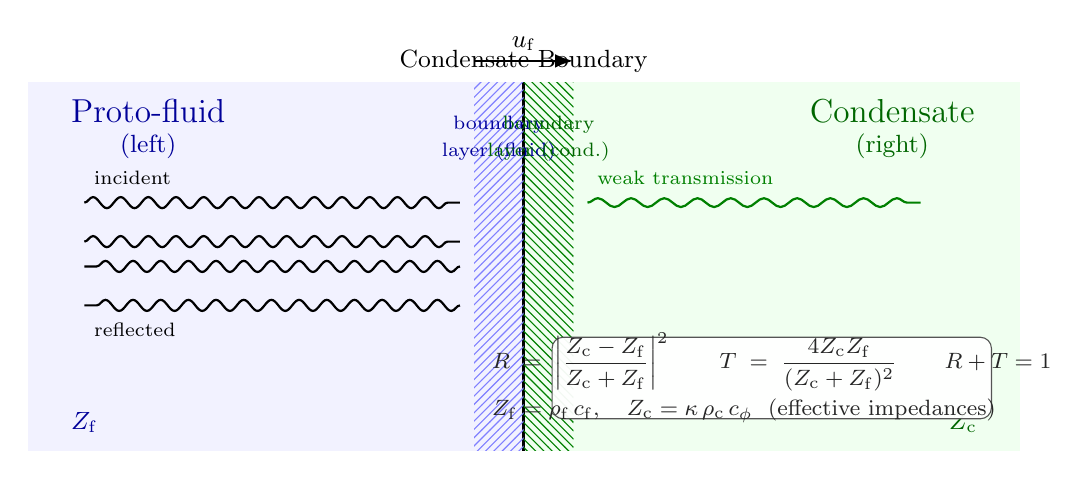
\begin{tikzpicture}[x=0.9cm,y=0.9cm,>=Latex]

  % -- REGIONS -------------------------------------------------------
  \fill[blue!5] (-7,-2.6) rectangle (0,2.6);   % Proto-fluid (left)
  \fill[green!6] (0,-2.6) rectangle (7,2.6);   % Condensate (right)

  % -- BOUNDARY & LAYERS --------------------------------------------
  \draw[very thick,black] (0,-2.6) -- (0,2.6); % Boundary line
  \node[black] at (0,2.9) {\small Condensate Boundary};
  \draw[->,thick] (-0.7,2.9) -- (0.7,2.9) node[midway,above]{\small $u_{\rm f}$};

  \def\BL{0.7} % boundary-layer half-width each side
  \fill[pattern=north east lines, pattern color=blue!50] (-\BL,-2.6) rectangle (0,2.6);
  \fill[pattern=north west lines, pattern color=green!50!black] (0,-2.6) rectangle (\BL,2.6);

  % -- LABELS (kept clear of formulas) -------------------------------
  \node[blue!60!black] at (-5.3,2.2) {\large Proto-fluid};
  \node[blue!60!black] at (-5.3,1.7) {\small (left)};
  \node[green!40!black] at (5.2,2.2) {\large Condensate};
  \node[green!40!black] at (5.2,1.7) {\small (right)};

  \node[blue!60!black,align=center] at (-0.35,1.8) {\scriptsize boundary\\[-2pt]\scriptsize layer (fluid)};
  \node[green!40!black,align=center] at (0.35,1.8) {\scriptsize boundary\\[-2pt]\scriptsize layer (cond.)};

  \node[blue!60!black] at (-6.2,-2.2) {\small $Z_{\rm f}$};
  \node[green!40!black] at (6.2,-2.2) {\small $Z_{\rm c}$};

  % -- WAVES ---------------------------------------------------------
  % Incident waves (left-to-right)
  \draw[thick,decorate,decoration={snake,amplitude=2pt,segment length=10pt}] (-6.2,0.90) -- (-0.9,0.90);
  \draw[thick,decorate,decoration={snake,amplitude=2pt,segment length=10pt}] (-6.2,0.35) -- (-0.9,0.35);
  \node[anchor=west] at (-6.2,1.25) {\scriptsize incident};

  % Reflected waves (right-to-left)
  \draw[thick,decorate,decoration={snake,amplitude=2pt,segment length=10pt}] (-0.9,0.00) -- (-6.2,0.00);
  \draw[thick,decorate,decoration={snake,amplitude=2pt,segment length=10pt}] (-0.9,-0.55) -- (-6.2,-0.55);
  \node[anchor=west] at (-6.2,-0.90) {\scriptsize reflected};

  % Weak transmitted wave in condensate
  \draw[thick,green!50!black,decorate,decoration={snake,amplitude=1.6pt,segment length=12pt}] (0.9,0.90) -- (5.6,0.90);
  \node[green!50!black,anchor=west] at (0.9,1.25) {\scriptsize weak transmission};

  % -- FORMULA BOX (below waves) ------------------------------------
  \begin{scope}
    \coordinate (boxSW) at (0.4,-2.15);
    \coordinate (boxNE) at (6.6,-1.0);
    \draw[rounded corners,black!70,fill=white,opacity=0.95] (boxSW) rectangle (boxNE);
    \node[align=left,black!85] at ($(boxSW)!0.5!(boxNE)$) {\footnotesize
      $R \;=\; \left|\dfrac{Z_{\rm c}-Z_{\rm f}}{Z_{\rm c}+Z_{\rm f}}\right|^{2}
      \qquad
      T \;=\; \dfrac{4 Z_{\rm c}Z_{\rm f}}{(Z_{\rm c}+Z_{\rm f})^{2}}
      \qquad
      R+T=1$\\[2pt]
      \footnotesize $Z_{\rm f}=\rho_{\rm f}\,c_{\rm f}, \quad
      Z_{\rm c}=\kappa\,\rho_{\rm c}\,c_{\phi} \ \ \text{(effective impedances)}$};
  \end{scope}

\end{tikzpicture}
\caption{\textbf{Advancing Condensate Boundary with two boundary layers and impedance mismatch.}
Waves in the proto‑fluid reach the boundary (vertical black line) and undergo refraction with strong reflection due to impedance mismatch ($Z_{\rm f}\!\neq\!Z_{\rm c}$). Hatched bands show the \emph{boundary layer (fluid side)} and the \emph{boundary layer (condensate side)}. Most power reflects; only a weak transmission enters the condensate. The situation is analogous to a \emph{P/N junction} depletion region: a built‑in barrier creates poor transmission and strong reflection, causing wave energy to build up at the interface.}
\label{fig:clean-boundary}
\end{figure}

\section{Condensate Boundary, Impedance Mismatch, and Boundary--Layer Compression}
As the condensate fills space, the \emph{Condensate Boundary} separates condensate from proto--fluid and advances with normal speed $u_{\rm f}$ (Fig.~\ref{fig:clean-boundary}). Because the effective wave impedances differ across the boundary, waves in the proto--fluid experience strong \emph{refraction with reflection}. In a scalar--wave analogue,
\be
Z_{\rm f}=\rho_{\rm f}\,c_{\rm f},\qquad
Z_{\rm c}=\kappa\,\rho_{\rm c}\,c_{\phi},
\ee
where $c_{\rm f}$ is the effective wave speed in the proto--fluid, $c_{\phi}$ the phase/phonon speed in the condensate, and $\kappa$ encodes coherence/coupling (dimensionless). The power reflection/transmission coefficients are
\be
R=\left|\frac{Z_{\rm c}-Z_{\rm f}}{Z_{\rm c}+Z_{\rm f}}\right|^{2},\qquad
T=\frac{4 Z_{\rm c}Z_{\rm f}}{(Z_{\rm c}+Z_{\rm f})^{2}},\qquad R+T=1.
\label{eq:RT}
\ee
For strong mismatch, $R\to 1$; in the boundary rest frame, modes also see a Doppler shift
\be
\omega' \simeq \omega - u_{\rm f}\,k_\parallel,\qquad
\gamma_{\rm comp} \sim \frac{1}{1-(u_{\rm f}/v_{\rm g})\cos\theta},
\ee
so that wavelengths shorten and energy density increases within the boundary layers. The picture is similar to a \emph{P/N junction} depletion region: a built‑in impedance barrier suppresses transmission and enhances reflection, producing local energy build‑up.

\section{Induced Gravity and the Role of the Energy Build--Up}
Even absent a bare EH term, integrating out fluctuations generates
\be
S_{\rm ind}[g]\supset \int \dx^4x\,\sqrt{-g}\;\frac{M_{\rm ind}^2}{2}\,R,\qquad
M_{\rm ind}^2\sim \sum_i \frac{N_i}{16\pi^2}\,\Lambda_{i,\rm eff}^2.
\ee
Boundary--layer compression increases the effective short--mode content $\Lambda_{i,\rm eff}$ transiently. For the \emph{expansion rate} $H(a)$ the dominant driver is the \emph{mechanical energy reservoir} $u_{\rm mech}(a)$ created by trapped/compressed waves; the small $M_{\rm ind}^2$ shift provides the CLF link but is assumed subdominant to respect BBN/CMB bounds.

\section{How Compression Boosts \texorpdfstring{$H(a)$}{H(a)}}
Model the reservoir as a narrow lognormal bump in $\ln a$:
\be
H^2(a)=\frac{8\pi G_0}{3}\Big[\rho_{\rm std}(a)+u_{\rm mech}(a)\Big],
\qquad
u_{\rm mech}(a)=\rho_{\rm c0}\,f_{\rm mech}\,
\exp\!\Big[-\frac{\ln^2(a/\ac)}{2\sigma^2}\Big],
\label{eq:Hboost}
\ee
with peak fraction $f_{\rm mech}\!\ll\!1$, center $\ac$ (typically $\zc\!\sim\!3000$--$5000$), and narrow width $\sigma\!\lesssim\!0.2$. Around the peak,
\be
\frac{\Delta H}{H}\;\approx\;\frac{1}{2}\,\frac{u_{\rm mech}(a)}{\rho_{\rm std}(a)}
\;\sim\;\frac{1}{2}\,f_{\rm mech}\,\frac{\rho_{\rm c0}}{\rho_{\rm std}(a)}\,
\exp\!\Big[-\frac{\ln^2(a/\ac)}{2\sigma^2}\Big].
\ee
A few--percent $f_{\rm mech}$ yields an $\mathcal{O}(2\text{--}5\%)$ rise in $H$ during a narrow window. The comoving sound horizon
\be
\rs=\int_0^{a_\ast}\frac{\cs(a)}{a^2 H(a)}\,\dx a,
\qquad
\cs(a)=\frac{c}{\sqrt{3\big(1+\tfrac{3}{4}\rho_b/\rho_\gamma\big)}},
\ee
then \emph{decreases} because $H(a)$ is larger near $\ac$. Fixing CMB peak angles implies a higher inferred $H_0$ once the model is fit, mirroring EDE logic \cite{EDEReview2023,PoulinReview2023,Planck2018}. After the boundary vanishes, $u_{\rm mech}\!\to\!0$ and late--time gravity is standard (including $c_T\!=\!c$ today \cite{GW170817}).

\section{Consistency Conditions and Practical Priors}
\paragraph{BBN.} Negligible modification at $T\!\sim$MeV: center the bump at $\zc\!\sim\!3000$ with narrow $\sigma$ and small amplitude (few percent bound) \cite{Alvey2020}.

\paragraph{CMB (Planck/ACT).} Keep the bump early and narrow to avoid damping--tail and phase distortions while still shrinking $\rs$ \cite{Planck2018,EDEReview2023,PoulinReview2023}.

\paragraph{Late--time gravity and GW170817.} Enforce $\Geff(a\!=\!1)\!=\!G_0$ and vanishing late tails; retain $c_T\!=\!c$ today \cite{GW170817}.

\section{Data--Facing Parameters and Test Plan}
Scan $\{\zc,\sigma,f_{\rm mech}\}$ (and optionally a small amplitude for an EH--prefactor bump) with Planck TT/TE/EE+lensing, BAO, Pantheon+/SNe, and SH0ES; test weak--lensing ($S_8$). The minimal reservoir form in Eq.\,\eqref{eq:Hboost} is designed for direct comparison to EDE analyses \cite{Planck2018,RiessReview2024}.

\section{Conclusions}
CF--BWC is the \emph{bridge} linking the CLF's mechanical stiffness to a controlled, early--time boost in $H(a)$. The advancing Condensate Boundary creates an impedance--mismatch interface where waves from the proto--fluid cannot efficiently transmit; they reflect, pile up, and compress in thin boundary layers, briefly creating an energy reservoir that boosts $H(a)$. A small, concurrent EH--prefactor shift provides the microphysical CLF link. The result is a short EDE--like episode that shrinks $\rs$ and raises the CMB--inferred $H_0$, then shuts off as the boundary disappears—thereby respecting BBN, CMB, late--time gravity, and GW170817 constraints.

\section*{Acknowledgments}
I thank colleagues in analogue gravity, quantum fluids, and cosmological inference for many helpful discussions.

\appendix
\section{One--Loop Induced Gravity: Intuitive Summary}
Even without a bare EH term, integrating out fluctuations in curved spacetime generates $\int \sqrt{-g}\,R$ with a coefficient controlled by the short--wavelength spectrum \cite{Sakharov1967,Vassilevich2003}. A moving boundary that traps and compresses waves temporarily increases short modes; the principal cosmological impact is the transient $u_{\rm mech}(a)$ that boosts $H(a)$, while any induced EH bump remains small to respect early--Universe bounds.

\section*{References}
\begin{thebibliography}{99}

\bibitem{Sakharov1967}
A.\,D.~Sakharov, ``Vacuum quantum fluctuations in curved space and the theory of gravitation,'' \emph{Sov. Phys. Dokl.} \textbf{12}, 1040 (1968).

\bibitem{Vassilevich2003}
D.\,V.~Vassilevich, ``Heat kernel expansion: User's manual,'' \emph{Phys. Rept.} \textbf{388}, 279--360 (2003).

\bibitem{Schwinger1951}
J.~Schwinger, ``On gauge invariance and vacuum polarization,'' \emph{Phys. Rev.} \textbf{82}, 664 (1951).

\bibitem{Planck2018}
Planck Collaboration, ``Planck 2018 results. VI. Cosmological parameters,'' \emph{Astron. Astrophys.} \textbf{641}, A6 (2020).

\bibitem{EDEReview2023}
M.~Kamionkowski and A.\,G.~Riess, ``The Hubble Tension and Early Dark Energy,'' \emph{Ann. Rev. Nucl. Part. Sci.} \textbf{73}, 153 (2023).

\bibitem{PoulinReview2023}
V.~Poulin, T.\,L.~Smith, T.~Karwal, ``The Ups and Downs of Early Dark Energy solutions to the Hubble tension,'' \emph{Phys. Dark Univ.} \textbf{42}, 101348 (2023).

\bibitem{RiessReview2024}
A.\,G.~Riess and L.~Breuval, ``The Local Value of $H_0$,'' arXiv:2308.10954 (2024).

\bibitem{GW170817}
B.\,P.~Abbott \emph{et al.}, ``Gravitational Waves and Gamma-Rays from a Binary Neutron Star Merger: GW170817 and GRB 170817A,'' \emph{Astrophys. J. Lett.} \textbf{848}, L13 (2017).

\bibitem{Alvey2020}
J.~Alvey, N.~Sabti, M.~Escudero, M.~Fairbairn, ``Improved BBN constraints on the variation of the gravitational constant,'' \emph{Eur. Phys. J. C} \textbf{80}, 148 (2020).

\end{thebibliography}

\end{document}